%-*- program: xelatex -*-        
%-*- program: biber -*-`        
%-*- program: xelatex -*-
\documentclass[11pt]{article}
\usepackage[margin=0.75in]{geometry}            % See geometry.pdf to learn the layout options. There are lots.
\geometry{letterpaper}  
\usepackage{amsmath,textcomp,amssymb,geometry,graphicx,enumerate,upquote,color}
\usepackage{hyperref}
\usepackage{breqn}
\usepackage{float}
\usepackage{tikz}
\usepackage{array}
\usepackage{float}
\usepackage{stfloats}
\usepackage{amsfonts}
\def\Session{Fall 2015}
\usepackage[english]{babel}
\title{Risk Measures and Serial Correlation}
\author{Boying Gong, Xinyue Zhou}
\newenvironment{qparts}{\begin{enumerate}[{(}a{)}]}{\end{enumerate}}
\def\endproofmark{$\Box$}
\newenvironment{proof}{\par{\bf Proof}:}{\endproofmark\smallskip}
\begin{document}
\maketitle

% \tableofcontents

% \clearpage

\begin{abstract}
Conditional Expected Drawdown (CED), the tail mean of maximum drawdown distribution, is a newly proposed positive homogenous and convex risk measure. Since maximum drawdown is defined as the accumulative loss from peak to trough, we expect CED to be inherently path dependent and account for serial correlation. Most currently widely-used risk measures such as Value at Risk (VaR), Expected Shortfall (ES) and volatility are based on daily returns and do not account for consecutive losses. We compared CED with these risk measures and show that CED is more sensitive to serial correlation on empirical and theoretical perspective. 
\end{abstract}

\section{Introduction}

Firms and regulators constantly quote risk measures such as VaR, ES and volatility to gauge the amount of asset needed for potential losses. These risk measures are usually calculated from the daily return distribution, thus only accounts for daily losses. However, during the events when consecutive losses happen such as 2008 financial crisis, these measures would become less informative due to the failure to consider the serial correlation of returns. Noticing this drawback of traditional risk measures, Goldberg and Mahmoud\cite{goldberg2014convex} developed Conditional Expected Drawdown (CED), a new risk measure defined over the empirical distribution of maximum drawdown. In this paper, we examine the relationship between serial correlation and various risk measures including CED. 

\subsection{Risk measures}

In the rest of the paper, we mainly focus on the comparison of CED and three extensively studied risk measures including Value at Risk (VaR), Expected Shortfall (ES) and volatility.

\begin{itemize}
\item $\textit{Conditional Expected Drawdown (CED)}$ is defined as the tail mean of maximum drawdown distribution.
\begin{equation}
CED_\alpha(X_{T_n}) = \mathbb{E}(\boldsymbol{\mu}(X_{T_n})|\boldsymbol{\mu}(X_{T_n}) > DT_\alpha).
\end{equation}
where $\alpha$ is the significance level, $DT_\alpha$ is the $\alpha$ quantile of maximum drawdown distribution, $\boldsymbol{\mu}(X_{T_n})$ represents $\textit{Maximum drawdown}$. In the return path of length n, the maximum drawdown is defined by
\begin{equation}
\boldsymbol{\mu}(X_{T_n}) = \mathrm{max_{1 < i < j \leq n} max}({X_{t_i}-X_{t_j}, 0}).
\end{equation}
Maximum drawdown is interpreted as the largest accumulative loss from peak to trough. For the detailed description of CED and its properties including path-dependency, convexity, and positive homogeneity, we direct the interested reader to Goldberg and Mahmoud\cite{goldberg2014convex}.


\item $\textit{Value at Risk (VaR)} $ estimates the potential loss of financial investment in a period. VaR is widely used by investment industry to assess the amount of assets needed to cover possible losses. For a given significant level $\alpha$, VaR is defined as the $\alpha$ quantile of the asset return distribution, which suggests the probability that the amount of loss excess VaR($\alpha$) is less than $\alpha$. The mathematical representation of VaR is: 
\begin{equation}
VaR_{\alpha}(L) = inf\{l \in \mathbb{R} : P(L > l) \leq 1-\alpha \} = 
inf\{l \in \mathbb{R} : F_L(l) \geq \alpha \}.
\end{equation}

\item $\textit{Expected shortfall (ES)}$ is a risk measure which resembles VaR but satisfies monotonicity, translation invariance, homogeneity and subadditivity. The ES of a financial asset is calculated as the tail mean of its return distribution. The Expected shortfall at level $\alpha$ is the expected value of loss which exceeds VaR($\alpha$). It is more sensitive to the shape of the loss distribution especially the tail of the distribution. The mathematical representation of ES is:
\begin{equation}
ES_{\alpha}(L) = E\left[ L \vert L<VaR_{\alpha}(L) \right].
\end{equation}

\item $\textit{Volatility}$ is measured by the standard deviation of asset returns. Higher volatility usually implies greater risk. Under the normality assumption of returns, volatility is proportional to VaR and ES. Although real world asset returns often have fatter tails than normal, volatility is often strongly correlated with VaR and ES, which we will see in later analysis. 

\end{itemize}

\subsection{Serial correlation}

Serial correlation, also known as autocorrelation, is the correlation of observations at different time point. Under the wide-sense stationary process assumption, the serial correlation of $X$ between two time point $t$ and $s$ can be measured by the autocorrelation function as follows:

\begin{equation}
R(\tau) = R(s, t) = \frac{E[(X_t-\mu)(X_s-\mu)]}{\sigma^2}.
\end{equation}

where $\tau = t-s$.

Serial correlation is often associated with the violation of efficiency market and random walk hypothesis. The literature documenting empirical serial correlation is extensive in the late 1980's\footnote{See Barucci and Emilio (2012, Section 6.5) \cite{barucci2012financial} for a detailed review.}. In stock price, Lo and MacKinlay (1988) \cite{lo1988stock} argue that returns based on the horizon longer than one year show a significant mean reversion, while Poterba and Summers (1988) \cite{poterba1988mean} detect a mean aversion for weekly and monthly returns. Lo and Mavkinlay (1988) \cite{lo1988stock}, Conrad et al. (1991) \cite{conrad1991components} model the security returns using a positively autocorrelated common component, an idiosyncratic component and a white-noise component. More extensively, the serial correlation has been documented in literature on nonsynchronous trading, which means assets are not traded simultaneously \cite{lo1990econometric}. Mech and Timothy (1993) \cite{mech1993portfolio} present evidence that the autocorrelation is associated with the delaying in price adjustment caused by transaction costs. In hedge fund returns, Getmansky, Lo and Makarov (2004) argue that serial correlation is an outcome of illiquidity exposure and smoothed returns, market inefficiencies, time-varying expected returns  and leverage and incentive fees with high water marks.

Assuming a moving average representation of reported returns, Getmansky, Lo and Makarov (2004) \cite{getmansky2004econometric} show that Sharp Ratio (SR) tends to be overstated and the market beta understated. Cesare, Stork and Vries (2014) \cite{di2014risk} use the similar structure to demonstrate that the reported value-at-risk (VaR) and expected shortfall (ES) are always smaller than or equal to their actual values. Thus, the risks of assets are easily underestimated using standard risk measures, and the investment decisions may be misleading. Although based on serial correlation and smoothing feature of hedge fund returns, their models are as well applicable to other assets with autocorrelated returns. 

\subsection{Synopsis}

The plan of the paper is as follows. In \emph{Part I: Empirical Analysis}, we present empirical studies analyzing daily returns of various assets. Section 2 provides overall and time-varying risk diagnostics stressing both correlation and the difference between CED and other risk measures. In Section 3, we relate serial correlation with risk measures by fitting time series models, includes AR, MA, ARMA and GARCH. In Section 4, we give an empirical analysis of risk contributions by constructing portfolios of different weights. Next in \emph{Part II: Simulations}, we further illustrate properties of CED by generating returns from time series models. Section 5 contains the comparison of risk measures of various models. And we also give the analysis of the relationship between serial correlation and risk measures based on simulated models. Finally in Section 7, we show that higher serial correlation would result in higher drawdown risk concentrations.

\part{Empirical Analysis}

In this part, we provide the empirical analysis for various asset classes including S\&P 500 Index (SPX), Russell 3000 Index (RAY), etc. Detailed descriptions of their date ranges, components, and summary statistics are given in Appendix \ref{App:AppendixA}.

\section{Risk diagnostics}

\subsection{Overall risk diagnostics}

Table \ref{table:Overall_risk} shows the overall values of four risk measures for various assets over their time range. For each of VaR, ES and CED, we present results of two significance levels 90\% and 95\%. Volatility, ES and VaR are on daily-scale to allow comparison between risk measures in the future. 

\begin{table}[bp]
\centering 
\begin{tabular}{ | r || p{1.5cm} | p{1cm} p{1cm} | p{1cm} p{1cm} | p{1cm} p{1cm} | p{1cm} p{1cm} | } 
 \hline
Measures & Volatility & \multicolumn{2}{c|}{VaR(\%)} & \multicolumn{2}{c|}{ES(\%)} &
 \multicolumn{2}{p{2cm}|}{CED(\%)\quad(3 month)} &\multicolumn{2}{p{2cm}|}{CED(\%)\quad(6 month)} \\ 
Levels & & 0.90 & 0.95 & 0.90 & 0.95 & 0.90 & 0.95 & 0.90 & 0.95 \\
  \hline \hline
AGG & 0.32 & 0.29 & 0.40 & 0.50 & 0.66 & 5.60 &  7.72 & 8.12 & 11.45  \\ 
HYG & 0.84 &  0.62 & 1.03 & 1.41 & 2.03 & 18.41 & 24.07 & 26.43 & 30.77 \\ 
TIP & 0.41 &  0.44 & 0.62 & 0.72 & 0.91 & 7.48 & 9.90 & 11.14 & 12.91 \\ 
BCOM & 0.94 &  1.04 & 1.47 & 1.71 & 2.20 & 18.14 & 22.54 & 26.61 & 33.66 \\ 
MXEA & 0.97 &  1.02 & 1.46 & 1.74 & 2.26 & 20.39 & 23.73 & 27.21 & 31.79 \\ 
MXEF & 1.13 &  1.21 & 1.76 & 2.11 & 2.75 & 26.21 & 30.80 & 36.35 & 43.30 \\ 
RAY & 1.09 &  1.11 & 1.62 & 1.95 & 2.56 & 20.65 & 25.64 & 27.81 & 34.08 \\ 
RMZ & 2.30 &  1.91 & 3.00 & 3.99 & 5.62 & 37.30 & 48.41 & 52.04 & 62.41 \\ 
SPX & 0.97 &  0.99 & 1.43 & 1.71 & 2.23 & 18.35 & 22.67 & 25.18 & 30.65 \\ 
USGG10YR & 1.27 & 1.26 & 1.95 & 2.28 & 2.99 & 23.28 & 28.11 & 32.78 & 39.00 \\
 \hline
\end{tabular}
\caption{Overall risk measures for various assets}
\label{table:Overall_risk}
\end{table}

Note that VaR and ES are calculated based on the empirical distribution of daily returns. Another commonly used method would be based on Gaussian distribution assumption. However, in our case where all asset returns are fat-tailed distributed, applying Gaussian distribution would lead to erroneous results. VaR and ES will be overestimated at a lower confidence level and underestimated at a higher level. This discrepancy phenomenon is rather obvious when the return distribution has an extremely fat tail. We include results assuming Gaussian distribution in Appendix A for comparison.
 
The choice of path length is crucial for CED calculation. As shown in Table \ref{table:Overall_risk}, the value of CED is sensitive to path length. Here we present the CED with rolling three month and six month periods. CED is an increasing function of significance level and path length. We recommend period length no longer than six month for CED estimation. Please refer to an in-depth exploration of behaviour of maximum drawdown distribution and the choice of path length in next subsection. Due to the similarity in definition between CED and ES, they share many features in the calculation. Thus, many ES calculation technique could be implemented for CED estimation. 

While volatility, VaR and ES are strongly correlated with each other across assets, CED has a comparatively weaker correlation with the other three. Note that the four risk measures do not give the same asset sequence from the largest to the least risky asset. Occasionally one risk measure indicates different order under different levels and path length. For example, CED indicates HYG has larger risk than SPX, but other three suggest the opposite comparison result. Moreover, the 6 month CED under 90\% level gives the different relative risk between HYG and BCOM with its counterpart under 95\% level. Notice that the reverse of relative risk suggested by same risk measure for distinct confidence level is more common for CED than for other risk measures.

Back to the economic implications of these risk values. Top three assets in Table \ref{table:Overall_risk} (AGG, HYG, TIP), which are comprised of US bonds, have the smallest risk among all asset class; RMZ, constructed by US equity REITs (Real Estate Investment Trust), have much greater risk than the others; MXEF (MSCI Emerging Market Index), reflecting the emerging market equities, have larger risk than MXEA (MSCI Developed Market Index).

\subsection{Time-varying risk diagnostics}

Time varying risk measures refer to risk measures based on fixed rolling windows. A series of risk measures is obtained. Risk at each time point is given by the past returns of a fixed length. Time-varying risk diagnostics enable us not only to compare risk across assets but to analyze risk for the same asset over time. 

\subsubsection{Maximum dradown distribution}

Unlike VaR and ES, the empirical distribution of maximum drawdown is more sensitive to the time length of measurement. Figure \ref{fig: dmaxdd_RMZ} shows the maximum drawdown of various assets for different path length (3 months, 6 months, 1 year, 2 years, 5 years) separately. As revealed in Figure \ref{fig: dmaxdd_RMZ}, maximum drawdown distribution tends to: a) have the larger mean and variance; b) be multi-mode; c) lack variability of values; d) center around several specific values when we move to longer periods. 

\begin{figure}[bp]
\centering 
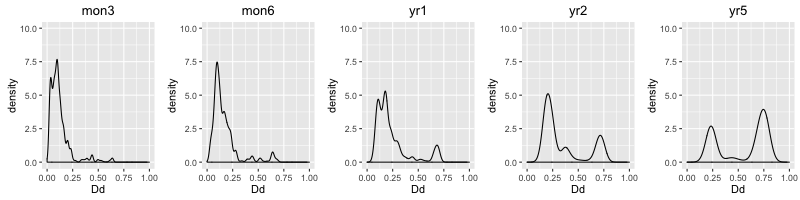
\includegraphics[width = 1\textwidth]{../results/maxdd_RMZ}
\caption{Maximum drawdown distribution of RMZ as rolling period increases} 
\label{fig: dmaxdd_RMZ}
\end{figure}

For daily return data, we do not recommend window length greater than six months for CED estimation. Large drawdowns in real-world asset returns are usually associated with particular events during a short time, for example, the 2008-2009 financial crisis. When considering longer path such as two years or five years, maximum drawdown values tend to be dominant by these events. The empirical distribution would only be defined on several distinct values. In such cases, the empirical quantile no longer exists without distributional or polynomial assumptions of the tail. Thus, it becomes hard to calculate the tail mean (CED). Later in our analysis, we use three or six-month path length. Figure \ref{fig: dist_mdd} shows the empirical distribution of maximum drawdown under the six-month rolling window for various assets.

\subsubsection{Time varying risk measures}

Under Gaussian distribution, VaR, ES, and volatility are linearly dependent. For empirical data where the return distribution has fat tails and distinct kurtosis, they are still strongly correlated. (With average correlation $>$ 95\% for six months rolling window) Figure \ref{fig: risk_meausre_RMZ} shows the VaR, volatility, ES, and maximum drawdown with rolling six-month periods. Four risk measures share a similar pattern of ups and downs, where the risk shot up during the 2008-2009 financial crisis. 

\begin{figure}
\centering 
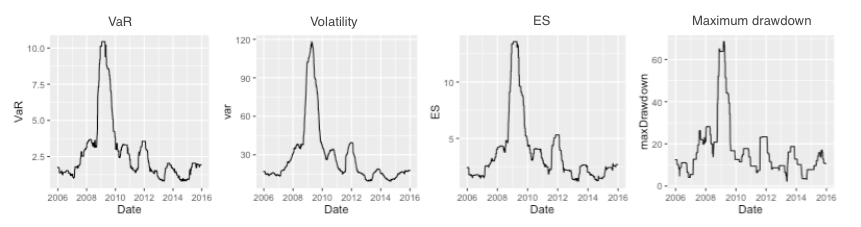
\includegraphics[width = 1\textwidth]{../results/risk_measure_RMZ}
\caption{Comparison of different risk measures of RMZ} 
\label{fig: risk_meausre_RMZ}
\end{figure}

\begin{figure}
\centering 
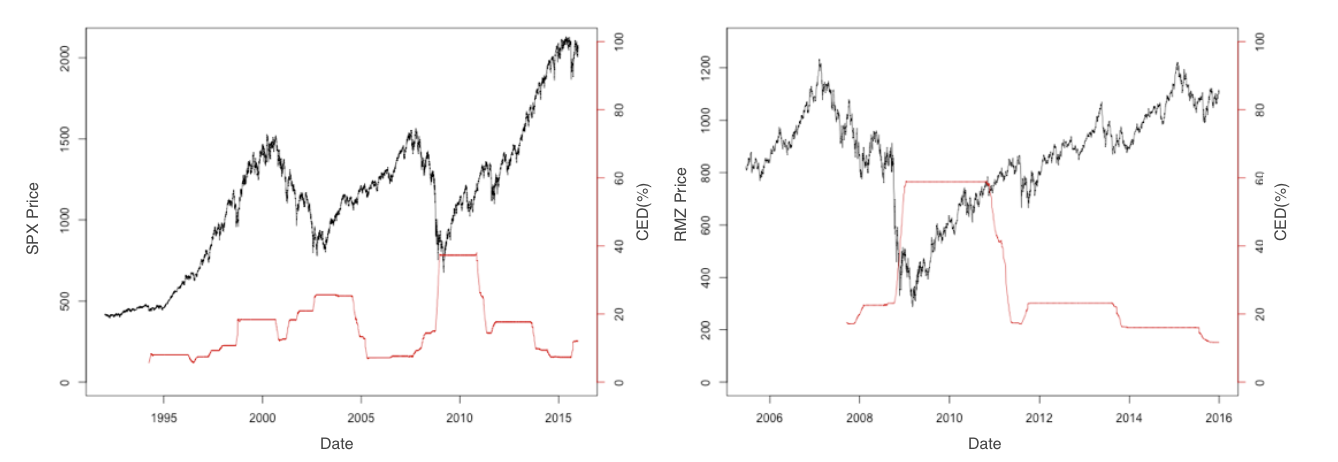
\includegraphics[width = 1\textwidth]{../figures/SPX_RMZ_P_CED}
\caption{Daily price of the S\&P 500 (SPX) and US equity REITs index (RMZ) togther with their 2-year-3month rolling CED.} 
\label{fig:SPX_RMZ_P_CED}
\end{figure}

CED requires more data compared with other risk measures and usually remain constant for a period. To empirically estimate the drawdown distribution, we often rolling a fixed path length. Credible quantile estimation requires hundreds of rollings. For example, two-year-three-month CED evaluates the three-month drawdown risk over the past two years. Figure \ref{fig:SPX_RMZ_P_CED} shows the daily price of the S\&P 500 (SPX) and US equity REITs Index (RMZ) together with their two-year-three-month rolling CED. The CED series also reflect the sharp increase in economic depressions.

CED is closely related to other risk measures. However, the correlation between CED and the other three risk measures are slightly weaker than the correlation among volatility, VaR, and ES. Table \ref{table:corrRiskMeasureCED} shows the correlation between CED and other risk measures calculated based on six-month rolling risk measures for every asset. 

\section{Time series analysis}

\subsection{ARMA}

\subsection{GARCH}

\subsection{Regime dependent analysis}



\subsection{Other return frequencies}

\section{Empirical risk contribution}


\part{Simulations}

\section{Serial correlation and risk measures}

\subsection{ARMA model}

\subsection{Garch model}

\subsection{Summary}




=========================================

AR, MA and ARMA model with normal dist and t dist, fat tail distribution would result in more randomness when calculating CED and other risk measures[Simulation Page 2 - 21]

Garch model fitting: how different coefficients influence the risk measure values? [Simulation Page 32]

Simulation with standard error adjusted [Simulation Page 21]

CED distinguishes negative from positive autocorrelation[Simulation Page 21]

Change standard deviation but fix everything in time series simulation would result in linear change of risk measures[Simulation Page 22]

The influence of volatility dominant in the risk measure calculation, relate this to empirical data, why usually we can not discover patterns? [To be added] 


\section{Risk contribution}






\newpage
\appendix
\section{Appendix A: Dataset} \label{App:AppendixA}
\subsection{Description}
\begin{table}[H]
\centering 
\begin{tabular}{ | r | p{7cm}  | p{4.5cm} | } 
 \hline 
Symbol & Name & Date range \\ \hline
AGG & iShares Core US Aggregate Bond & 2003-09-29 to 2015-12-31 \\
HYG & iShares iBoxx High Yield Corporate Bond & 2007-04-12 to 2015-12-31 \\
TIP & iShares TIPS Bond & 2003-12-08 to 2015-12-31 \\
BCOM & Bloomberg Commodity Index & 1991-01-03 to 2015-12-31 \\
G0O1 & 3-Month U.S. Treasury Bill Index & 1992-04-01 to 2015-12-31 \\
MXEA & MSCI Developed Markets Index & 1970-01-07 to 2015-12-31 \\
MXEF & MSCI Emerging Markets Index & 1988-01-01 to 2015-12-31 \\
RAY & Russell 3000 Index & 1979-01-02 to 2015-12-31 \\
RMZ & MSCI US REIT Index & 2005-06-20 to 2015-12-31 \\
SPX & S\&P 500 Index & 1950-01-04 to 2015-12-31 \\
USGG10YR & US Generic Govt 10 Year & 1962-01-03 to 2015-12-31 \\
 \hline
\end{tabular}
\caption{Normal VaR and ES under various levels}
\label{table:AssetDescription}
\end{table}


\subsection{Statistical summary}
annualized return, Sharpe Ratio, standard deviation, skewness, kurtosis [Empirical Page 8]

\subsection{Return}
Return across time and Return distribution [Empirical Page 8]

\subsection{Normal VaR and ES}

\begin{table}[H]
\centering 
\begin{tabular}{ | r || p{1cm} p{1cm} p{1cm} || p{1cm} p{1cm} p{1cm} | } 
 \hline
 & & VaR(\%) &&& ES(\%) & \\
Asset& 0.90 & 0.95 & 0.99 & 0.90 & 0.95 & 0.99 \\
  \hline \hline
AGG & 0.39 & 0.51 & 0.72 & 0.57 & 0.67 & 0.86\\ 
HYG & 1.06 & 1.36 & 1.94 & 1.50 & 1.76 & 2.26\\ 
TIP & 0.51 & 0.66 & 0.94 & 0.74 & 0.86 & 1.11\\ 
BCOM & 1.20 & 1.54 & 2.18 & 1.65 & 1.94 & 2.50\\ 
MXEA & 1.22 & 1.57 & 2.24 & 1.74 & 2.04 & 2.62\\ 
MXEF & 1.42 & 1.83 & 2.61 & 2.03 & 2.38 & 3.06\\ 
RAY & 1.36 & 1.75 & 2.49 & 1.95 & 2.29 & 2.94\\ 
RMZ & 2.92 & 3.75 & 5.32 & 4.08 & 4.79 & 6.18\\ 
SPX & 1.21 & 1.57 & 2.22 & 1.73 & 2.03 & 2.61\\ 
USGG10YR & 1.62 & 2.08 & 2.95 & 2.23 & 2.62 & 3.39\\
 \hline
\end{tabular}
\caption{Normal VaR and ES under various levels}
\label{table:VaRESNormal}
\end{table}



\section{Appendix B: Rolling risk diagnostics} \label{App:AppendixB}

\begin{figure}[H]
\centering
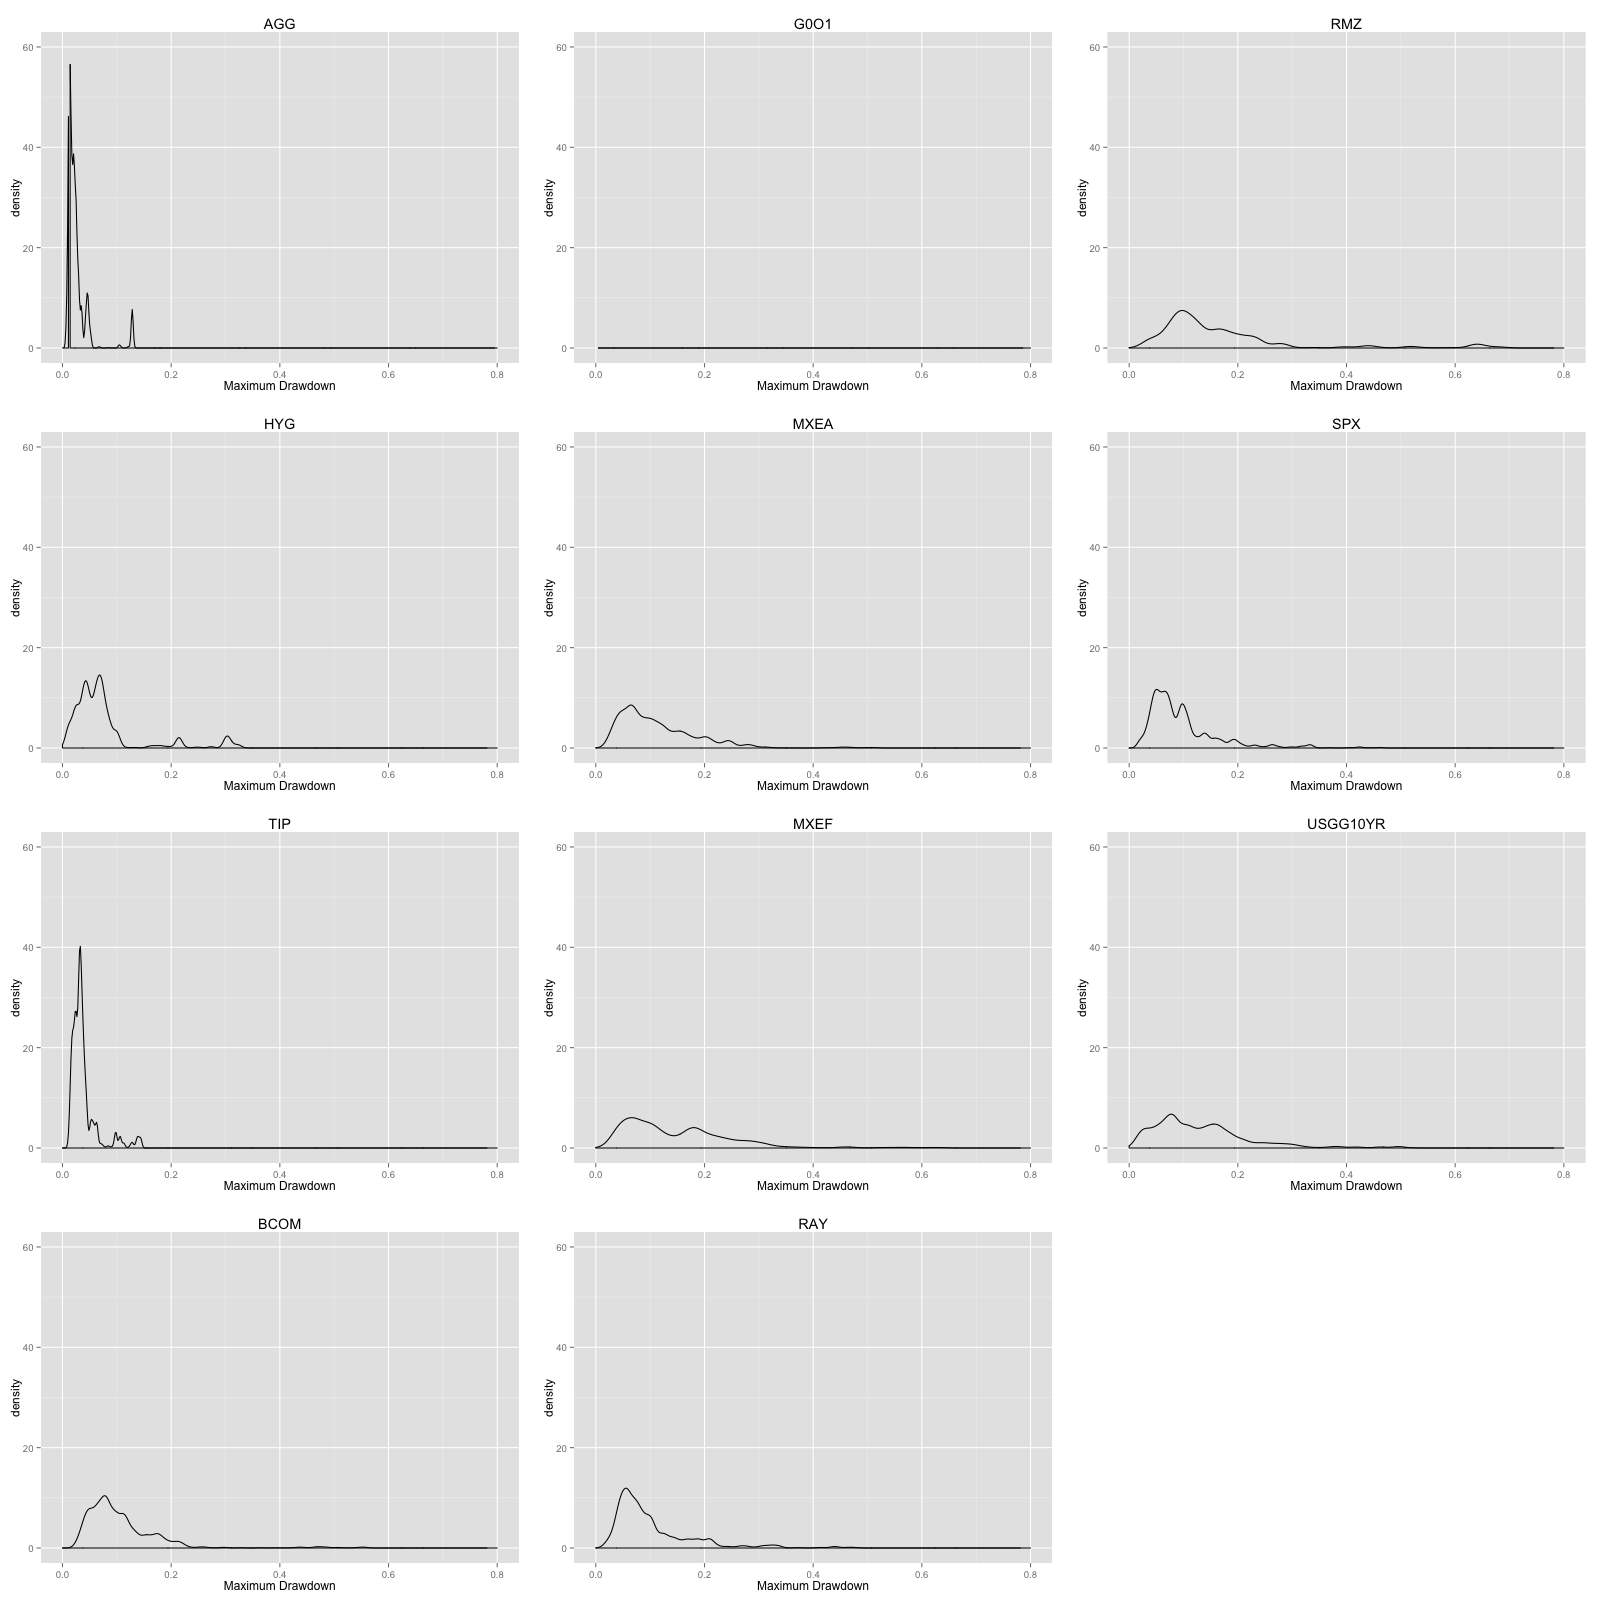
\includegraphics[width=15cm]{../results/maxdd_dist_mon6}
\caption{Empirical distribution of maximum drawdown under 6 month rolling window} 
\label{fig: dist_mdd}
\end{figure}

\begin{table}
\caption{Correlation between CED (confidence level = 0.9) and other risk measures}
\centering 
\begin{tabular}{| p{2cm}||p{2cm}|p{2cm}|p{2cm}|} 
\hline
Measures & Volatility & VaR & ES\\
  \hline
AGG & 0.94 & 0.89 & 0.95\\ 
HYG & 0.98 & 0.97 & 0.97\\ 
TIP & 0.77 & 0.85 & 0.85\\ 
BCOM & 0.84 & 0.89 & 0.89\\ 
MXEA & 0.84 & 0.83 & 0.86\\ 
MXEF & 0.91 & 0.91 & 0.93\\ 
RAY & 0.92 & 0.85 & 0.92\\ 
RMZ & 0.96 & 0.96 & 0.97\\ 
SPX & 0.84 & 0.81 & 0.84\\ 
USGG10YR & 0.91 & 0.93 & 0.95\\
\hline
\end{tabular}
\label{table:corrRiskMeasureCED}
\end{table}

\newpage

\bibliographystyle{unsrt}
\bibliography{analysis}






\clearpage


===========Overall risk measures for various assets============

(Use unannualized VaR, ES and volatility in order to compare)

VaR, ES: Empirical method \& normal method, VaR and ES is being overestimated at a lower confidence level and being underestimated at a higher confidence level. [Empirical, Page 49]

Volatility: [Empirical, Page 8]

Overall CED: how they are different under different confidentce interval and rolling windows [Empirical, Page 10]

Relationship between risk measures: assets with larger VaR, ES and volatility also have larger CED, give the correlation values, Do they give the same order from lowest risk asset to highest?[Empirical, Page 10]

Asset with largest and smallest risk for each risk measures: relate this with intuitive sence and the component of asset class. [Empirical, Page 9]

Relative values of different assets for different risk measures: Is there a risk measure distinguish assets from each other most? [To be added]


===========Time-varying risk diagnostics=============

Empirical distribution of maximum drawdown is sensitive to the time length of measurement. [Empirical, Page 11, Figure 1]

Large windows not desirable, why? [Empirical, Page 11, 13, Figure 1; Presentation2 Page3]

Correlation between risk measures over time [Empirical, Table 4, 5, Figure 2, 27]

CED plot

Risk measures, when biggest? related to real world events. [To be extended]

=============== regime switching model ======

Introduction [Summary Page 13]

Summary of regime switching model for different assets [Summary Page 13][To be add: modeled variance]

Why can not see strong correlation between serial correlation and CED? Relate this to the simulation study: when both volatility and seiral correlation are different, volatility usually dominant the influence for CED. [To be added]

Rolling risk measure (RMZ as example): Correlation between seial correlation and risk measure for two regions [Empirical Page 15]

==============================================

Which model gives the best fit (statistically)? Which assets have strongest serial correlation? The point here is to to understand the autocorrelation behavior of vaious asset classes, so you should once again interpret your results and parameters.

relationship of the time series of the serial correlation parameters (e.g. $\kappa$ in the AR(1) model) with the time series of the various risk diagnostics. Is serial correlation strongly related to volatility, ES, VaR and CED? Is it more strongly correlated to one risk measure than another?



Part I: Empirical analysis

1. Understand the different risk characteristics (particularly drawdown) of different asset classes.

2. Comparing the insights gained by looking at the maximum drawdown distribution in addition to the returns distribution.

3. Find the empirical relationship between serial correlation and risk.


Part II: Simulations

1. Comparison of risk measures of various simulated models.

2. Comparison of the returns and maximum drawdown distribution for various simulated models. (parallel to point 2 above)

3. Relationship between serial correlation and risk based on simulated models. (parallel to point 3 above)


The answer is that simulation and empirical analysis are two elements that play a complementary role in our understanding of the financial world, and specifically of drawdown risk: empirical analyses roughly guide us in understanding what are economically reasonable assumptions. Simulations help us estimate models from data generated by a known process. These simulated models are often used in practice for the purpose of forecasting and are tested out-of-sample for accuracy on empirical data. (Note however that forecasting will not be part of your project.)


Our hypothesis for this next part is that higher serial correlation would result in higher drawdown risk concentrations (compared with risk concentrations along the other risk measures). Here is an outline of what you can do:

1. Simulate the returns to two assets E (representing equity) and B (representing Bonds). For each model you simulate (AR, MA, GARCH, combination models, etc), you can use the parameters obtained by fitting to the real time series of equity and bonds (which you already have). Moreover, if your error term is Gaussian, you could use the real volatility of the underlying assets for the simulation.

2. For each model you simulate, construct 50/50, 60/40, and 70/30 portfolios.

3. For each model and portfolio, calculate the overall fractional risk contributions to volatility, ES, and CED along assets E and B.



\end{document}